\chapter{Preliminaries}
\label{chapter:preliminaries}

%%%%%%%%%%%%%%%%%%%%%%%%%%%%%%%%%%%%%%%%%%%%%%%%%%%%%%%%%%%%%%%%%%%%%%%%%%%%%%%%
%                                                                              %
%%%%%%%%%%%%%%%%%%%%%%%%%%%%%%%%%%%%%%%%%%%%%%%%%%%%%%%%%%%%%%%%%%%%%%%%%%%%%%%%

\section{Metric First-Order Temporal Logic}
\label{section:mfotl}

Metric First-Order Logic (MFOTL)
\cite{basin2015monitoring, chomicki1995efficient}
combines first-order predicate logic with temporal operators such as
$\Next$ ("next"), $\Prev$ ("previous"), $\UUntil$ ("until"), and $\Since$ ("since").
MFOTL is frequently used as a policy language in
runtime verification \cite{whyenf, lex, basin2015monitoring}.

\begin{definition}
    \label{def:mfotl-signature}
    An \emph{MFOTL Signature}
    $\Sigma = (\Domain, \Events, \Functions, \iota)$
    is a quadruple consisting of
    a value domain $\Domain$,
    a set of event names $\Events$,
    a set of function names $\Functions$,
    and an arity function $\iota : \Events \cup \Functions \to \Nat$.
\end{definition}
Definition \ref{def:mfotl-signature} is the the same signature
definition as in Hublet et. al \cite[Section 2.2.2]{lex}
and Hublet et. al \cite[Section 2]{whyenf}.
\begin{example}
    % TOOD: formatting
    \label{ex:signature}
    For
    \begin{align*}
        \Domain &= \texttt{strings} \cup \{ \bot, \top \} \cup \Nat, \\
        \Events &= \{ \mathsf{giveEmailConsent},
                      \mathsf{revokeEmailConsent},
                      \mathsf{sednEmail}
                      \}, \\
        \Functions &= \{ \mathsf{ageOfUser} \} \\
        \iota(\mathsf{giveEmailConsent}) &= 2, \\ % arguments: user, purpose
        \iota(\mathsf{revokeEmailConsent}) &= 2, \\ % arguments: user, purpose
        \iota(\mathsf{sendEmail}) &= 2, \\ % arguments: user, purpose
        \iota(\mathsf{ageOfUser}) &= 1
    \end{align*}
    $\Sigma = (\Domain, \Events, \Functions, \iota)$
    is an MFOTL signature.
\end{example}

\begin{definition}
    \label{def:event}
    An \emph{Event} is a tuple
    $(e, \left(p_1, \dots, p_k \right) )
    \in \Events \times \Domain^{k}$
    where $k=\iota(e)$ and all $p_i \in \Domain$.
\end{definition}
\begin{example}
    \label{ex:event}
    \begin{align*}
        &\mathsf{giveEmailConsent}(\text{"Alice"}, \text{"Account Updates"})
        \text{ and } \\
        &\mathsf{revokeEmailConsent}(\text{"Bob"}, \text{"Marketing"})
    \end{align*}
    are events over the signature $\Sigma$ from Example
    \ref{ex:signature}.
\end{example}

\begin{definition}
    \label{def:database}
    A \emph{Database} $D \in \Databases$ is a set of events.
\end{definition}

\begin{definition}
    \label{def:trace}
    A \emph{Trace} $\sigma \in \Traces$ is a sequence
    $\Sequence[1 \leq i \leq k]{(\tau_i, D_i)}$, $k \in \Nat \cup \lbrace \infty \rbrace$
    of timestamps $\tau_i \in \Nat$ and finite databases $D_i \in \Databases$,
    where timestamps grow \emph{monotonically}
    ($\forall i < |\sigma|.\,\tau_i \leq \tau_{i+1}$)
    and \emph{progress}
    (if $|\sigma| = \infty$, then $\lim_{i\to\infty} \tau_i = \infty$).
\end{definition}

\begin{definition}
    \label{def:infinite-trace}
    The set of \emph{Infinite Traces} is denoted by
    \begin{equation*}
        \Traces_\omega
        \subseteq 
        \left(
        \Nat \times \Databases
        \right)^{\infty}
    \end{equation*}
\end{definition}

\begin{definition}
    \label{def:finite-trace}
    The set of \emph{Finite Traces} is denoted by
    \begin{equation*}
        \Traces_f
        \subseteq 
        \left(
        \Nat \times \Databases
        \right)^*
    \end{equation*}
\end{definition}

\begin{definition}
    \label{def:time-point}
    A \emph{time-point} $0 \leq i \leq |\sigma|$ is an index in a trace $\sigma$.
\end{definition}

\begin{example}
    \label{ex:trace}
    \begin{align*}
        \sigma =
        \langle
        &(0, &&\{\mathsf{giveEmailConsent}(\text{"Alice"}, \text{"Account Updates"})\}), \\
        &(1, &&\{\mathsf{giveEmailConsent}(\text{"Bob"}, \text{"Marketing"})\}), \\
        &(2, &&\{\mathsf{revokeEmailConsent}(\text{"Alice"}, \text{"Account Updates"}), \\
             &&&\mathsf{giveEmailConsent}(\text{"Bob"}, \text{"Account Updates"})\}), \\
        &(10, &&\emptyset)
        \rangle
    \end{align*}
    $\sigma$ is a finite trace over the signature $\Sigma$ from Example
    \ref{ex:signature} with 4 time-points.
    The 4 time-points have the timestamps $0$, $1$, $2$, and $10$.
\end{example}
Traces like Example \ref{ex:trace} can be seen as representing
a system's behavior in a standardized form.

\begin{definition}
    \label{def:empty-trace}
    The \emph{Empty Trace} is denoted by $\emptytrace$.
\end{definition}

\begin{definition}
    \label{def:first-time-stamp}
    The function $\fts : \Traces \to \Nat \cup \left\{ \bot \right\}$
    gives the first time stamp in a trace unless it is empty.
    \begin{align*}
        \fts(\sigma) :=
        \begin{cases}
            \bot & \text{if } \sigma = \emptytrace \\
            \tau & \text{if } \sigma = \left( \tau, D \right) \cdot \sigma'
        \end{cases}
    \end{align*}
\end{definition}
\begin{definition}
    \label{def:last-time-stamp}
    The function $\lts : \Traces \to \Nat \cup \left\{ \bot \right\}$
    gives the first time stamp in a trace unless it is empty.
    \begin{align*}
        \lts(\sigma) :=
        \begin{cases}
            \bot & \text{if } \sigma = \emptytrace \\
            \tau & \text{if } \sigma = \sigma' \cdot \left( \tau, D \right)
        \end{cases}
    \end{align*}
\end{definition}
For the trace $\sigma$ in Example \ref{ex:trace} we have
$\fts(\sigma) = 0$ and $\lts(\sigma) = 10$.

\begin{definition}
    \label{def:property}
    A \emph{Property} is a subset $P\subseteq \Traces_\omega$.
\end{definition}

A Property can be induced by some policy $\phi$, we denote this policy by $P(\phi)$.
We say a trace $\sigma$ is compliant with policy $\phi$ if and only if $\sigma \in P(\phi)$.

\begin{definition}
    \label{def:non-empty-intervals}
    The set of \emph{Non-Empty Intervals} over $\Nat$ is denoted by $\Intervals$.
\end{definition}

Figure \ref{fig:mfotl-term-typing-rules} defines the rules for when an MFOTL
term is well-typed.
And Figure \ref{fig:mfotl-typing-rules} defines when an
MFOTL formula is well-typed.
In particular, these two sets of typing rules ensure that
all events and functions have the correct number of arguments.
Next we introduce the specific MFOTL grammar used 
which includes the notable additions of non-recursive
let-bindings \cite{zingg2022verified} and aggregations
\cite{basin2013monitoring}.
From here on let $\Variables$ be a set of variables.
The following grammar definition is the same as in 
Hublet et al. \cite[Section 2.2]{whyenf-2}.

\begin{definition}
    \label{def:mfotl-grammar}
    Let $c \in \Domain$,
    $x \in \Variables$,
    $f \in \Functions$,
    $e \in \Events$,
    and $I \in \Intervals$.
    Then our \emph{MFOTL Grammar} is defined by the following two rules
    \begin{align*}
        t &::= &&c \mid x \mid f(t,\dots,t) \\
        \phi &::= &&\top \mid e(t,\dots,t) \mid t=t \mid \neg \phi \mid
            \phi \wedge \phi \mid \exists.\ \phi \mid \Next_I \phi \mid
            \Prev_I \phi \mid \phi \UUntil_I \phi \mid \phi \Since_I \phi \\
            &&& \mid \Aggreg{x}{\omega}{t}{x,\dots,x}{\phi} \mid
            \LLet{e \left(x,\dots,x \right)}{\phi}{\phi}
    \end{align*}
\end{definition}

\begin{figure}
    \begin{gather*}
        \prftree[r]{Constant}
            {c \in \Domain}
            {\Gamma \vdash_{trm} c} \qquad
        \prftree[r]{Variable}
            {v \in \Variables}
            {\Gamma \vdash_{trm} v} \\
        \prftree[r]{Function}
            {f \in \Functions}
            {t_i \in \Domain}
            {\iota(f) = k}
            {\Gamma \vdash_{trm} f\left(t_1,\dots,t_k\right)}            
    \end{gather*}
    \vspace{-2em}
    \caption{MFOTL Term Typing Rules \label{fig:mfotl-term-typing-rules}}
\end{figure}

\begin{figure}
    \begin{gather*}
        \prftree[r]{True}
            {}
            {\Gamma \vdash \top} \qquad
        \prftree[r]{Not}
            {\Gamma \not\vdash \phi}
            {\Gamma \vdash \neg \phi} \qquad
        \prftree[r]{And}
            {\Gamma \vdash \phi}{\Gamma \vdash \psi}
            {\Gamma \vdash \phi \wedge \psi} \\
        \prftree[r]{Event}
            {e \in \Events}
            {\Gamma \vdash_{trm} x_i}
            {\Gamma \vdash e\left(x_1, \dots, x_k\right)} \qquad
        \prftree[r]{Exists}
            {\Gamma \vdash \phi}{x \in \Variables}
            {\Gamma \vdash \exists x. \phi} \\
        \prftree[r]{Next}
            {\Gamma \vdash \phi}{I \in \Intervals}
            {\Gamma \vdash \Next_I \phi} \qquad
        \prftree[r]{Previous}
            {\Gamma \vdash \phi}{I \in \Intervals}
            {\Gamma \vdash \Prev_I \phi} \\
        \prftree[r]{Until}
            {\Gamma \vdash \phi}{\Gamma \vdash \psi}{I \in \Intervals}
            {\Gamma \vdash \phi \UUntil_I \psi} \qquad
        \prftree[r]{Since}
            {\Gamma \vdash \phi}{\Gamma \vdash \psi}{I \in \Intervals}
            {\Gamma \vdash \phi \Since_I \psi} \\
        % \prftree[r]{Aggregation} % TODO: what are the typing rules for aggregation?
        %     {\Gamma \vdash \phi}{x \in \Variables }{\bar{y} \text{ TODO}}
        %         {t \text{ TODO}}{\omega \text{ TODO}}
        %     {\Gamma \vdash \Aggreg{x}{\omega}{t}{y_1,\dots,y_k}{\phi}} \\
        \prftree[r]{Let}
            {\Gamma \vdash \phi}
            {\Gamma
                [\Events \mapsto \Events \cup \lbrace e \rbrace,
                \iota \mapsto \iota[e \mapsto k]]
                \vdash \psi}
            {\Gamma \vdash_{trm} x_i}
            {\Gamma \vdash \LLet{e\left(x_1, \dots, x_k \right)}{\phi}{\psi}}
    \end{gather*}
    \vspace{-2em}
    \caption{MFOTL Typing Rules \label{fig:mfotl-typing-rules}}
\end{figure}


\begin{definition}
    \label{def:mfotl-valuation}
    A variable \emph{Valuation} $v: \Variables \to \Domain$
    assigns a value to a variable.
\end{definition}

\begin{definition}
    \label{def:mfotl-evaluation}
    The \emph{Evaluation} of well-typed MFOTL terms $t$ under some valuation $v$ is (recursively) defined as followed:
    \begin{align*}
        &\downarrow_v c
            &&:= c
            && \text{for all constants } c \in \Domain\\
        &\downarrow_v x
            &&:= v(x)
            && \text{for all variables } v \in \Variables\\
        &\downarrow_v f\left(t_1,\dots,t_k\right)
            &&:= \hat{f}\left(\downarrow_v t_1, \dots \downarrow_v t_k \right)
            && \text{for all functions } f \in \Functions \text{ and all terms } t_i
    \end{align*}
\end{definition}

\begin{definition}
    \label{def:mfotl-satisfaction}
    An MFOTL formula $\phi$ is \emph{satisfied} at some time-point $i$ in
    a trace $\sigma$ under
    some valuation $v$ is denoted by $v,i \vDash_\sigma \phi $.
\end{definition}
If the trace is obvious from context the subscript $\sigma$ in $\vDash_\sigma$ can be
omitted.
\begin{definition}
    \label{def:mfotl-semantics}
    The \emph{Semantics of MFOTL} for a fixed, infinite trace $\sigma$ is defined as followed
    \begin{align*}
        v, i &\vDash  \top \\
        v, i &\vDash  \neg \phi
            &&\text{iff } v, i \not\vDash  \phi \\
        v, i &\vDash  \phi \wedge \psi
            &&\text{iff } v, i \vDash  \phi \text{ and } v, i \vDash  \psi \\
        v, i &\vDash  e(t_1, \dots, t_k)
            &&\text{iff } e(\downarrow_v t_1, \dots, \downarrow_v t_k) \in D_i \\
        v, i &\vDash  \exists x. \phi
            &&\text{iff } v[x \mapsto d], i \vDash  \phi \text{ for some } d \in \Domain \\
        v, i &\vDash  \Next_I \phi
            &&\text{iff } v, i+1 \vDash  \phi \text{ and } \tau_{i+1} - \tau_i \in I \\
        v, i &\vDash  \Prev_I \phi
            &&\text{iff } i>0 \text{ and } v, i-1 \vDash  \phi
            \text{ and } \tau_i - \tau_{i-1} \in I \\
        v, i &\vDash  \phi \UUntil_I \psi
            &&\text{iff } v, j \vDash  \psi \text{ for some } j \geq i
            \text{ with } \tau_j - \tau_i \in I \\
            &&&
            \text{ and } v, k \vDash  \phi \text{ for all } i \leq k < j \\
        v, i &\vDash  \phi \Since_I \psi
            &&\text{iff } v, j \vDash  \psi \text{ for some } j \leq i
            \text{ with } \tau_i - \tau_j \in I \\
            &&&
            \text{ and } v, k \vDash  \phi \text{ for all } j < k \leq i \\
        % v, i &\vDash  \Aggreg{x}{\omega}{t}{y_1, \dots, y_k}{\phi}
        %     &&\text{iff } TODO \dots % TODO:
        % \\
        v, i &\vDash  \LLet{e(x_1, \dots, x_k)}{\phi}{\psi}
            && \text{iff } v, i \vDash_{\sigma \left[ \forall j. D_j \mapsto D_j \cup \left\lbrace e\left(\bar{d}\right) \mid v\left[\bar{x} \mapsto \bar{d}\right], j \vDash \phi \right\rbrace \right]} \psi
    \end{align*}
    
    Where $c \in \Domain$,
    $x \in \Variables$,
    $f \in \Functions$,
    $e \in \Events$,
    and $I \in \Intervals$.
    
\end{definition}

We define the following operators based on the basic operators above as
"syntactic sugar".
\begin{definition}
    \label{def:mfotl-syntactic-sugar}
    \emph{MFOTL Syntactic Sugar}
    \begin{align*}
        \bot &:= \neg\top &
        \phi \to \psi &:= \neg \phi \vee \psi \\
        \phi \vee \psi &:= \neg(\neg\phi \wedge \neg\psi) &
        \phi \leftrightarrow \psi
            &:= (\phi \to \psi) \wedge (\psi \to \phi) \\
        \forall x. \phi &:= \neg(\exists x. \neg \phi) \\
        \Eventually_I \phi &:= \top \UUntil_I \phi \quad \text{(eventually)} &
        \Once_I \phi &:= \top \Since_I \phi \quad \text{(once)}\\
        \Always_I \phi &:= \neg \Eventually \neg \phi \quad \text{(always)} &
        \Historically_I \phi &:= \neg \Once_I \neg \phi \quad \text{(historically)}
    \end{align*}    
\end{definition}

% TODO: possibly include definition of MFOLT language
\begin{definition}
    \label{def:mfotl-formula-language}
    The \emph{Language} of a MFOTL formula $\phi$ is
    $$
    \Language(\phi)
    = \left\lbrace
    \sigma \in \Traces_\omega \mid \exists v. v,0 \vDash \sigma
    \right\rbrace
    $$
\end{definition}

\begin{example}
    \label{ex:mfotl-formula}
    An example of an MFOTL formula over the signature $\Sigma$ from Example
    \ref{ex:signature} is
    \begin{align*}
        \phi := 
        &\Always_{[0,\infty)}(
            \mathsf{sendEmail}(\mathsf{user}, \text{"marketing"}) 
            \to \\
            & \quad ( \Once_{[0,\infty)} 
                \mathsf{giveEmailConsent}(\mathsf{user}, \text{"marketing"})
                \wedge \\
                & \quad
                (\neg
                \mathsf{revokeEmailConsent}(\mathsf{user}, \text{"marketing"})) \\
                & \qquad
                \Since_{[0,\infty)}
                \mathsf{giveEmailConsent}(\mathsf{user}, \text{"marketing"})
            )
        )
    \end{align*}
\end{example}
In words, this policy states that whenever an email is sent
to a user for marketing purposes, the user must have previously
given consent for receiving marketing emails and must not have revoked
this consent since then.

%%%%%%%%%%%%%%%%%%%%%%%%%%%%%%%%%%%%%%%%%%%%%%%%%%%%%%%%%%%%%%%%%%%%%%%%%%%%%%%%
%                                                                              %
%%%%%%%%%%%%%%%%%%%%%%%%%%%%%%%%%%%%%%%%%%%%%%%%%%%%%%%%%%%%%%%%%%%%%%%%%%%%%%%%
\section{Runtime Verification}
\label{section:runtime-verification}
Runtime Verification concerns itself with the behavior of
some System under Scrutiny (SuS) with regards to some policy.
Runtime Verification can be split into two related techniques: 
Runtime Monitoring and Runtime Enforcement.

\emph{Runtime Monitoring} is used to detect a policy violation either in an
online (real-time) or offline fashion.
In Runtime Monitoring a monitor continuously evaluates the current and past
system state and determines whether or not it complies with some policy.
For our purposes the system state gets abstracted into a trace of events
and the policy represents a set of allowed traces.
Since the monitor never interacts with the system itself, runtime
monitoring can also be done after a program has finished executing.
% TODO

\emph{Runtime Enforcement}
is used to actively cause or prevent certain system behaviors.
Due to this interactive nature of runtime enforcement it is inherently online.
If we consider our trace model on a high level, an enforcer can "edit" any
time-point before it gets fully committed to the trace and additionally
the enforcer can create its own time-points at any increment of time.
% TODO
The following subsection explores an approach for enforcing MFOTL policies.

%%%%%%%%%%%%%%%%%%%%%%%%%%%%%%%%%%%%%%%%%%%%%%%%%%%%%%%%%%%%%%%%%%%%%%%%%%%%%%%%
\subsection{Proactive Runtime Enforcement using MFOTL}
\label{subsection:proactive-runtime-enforcement}

\begin{figure}
    \begin{center}
        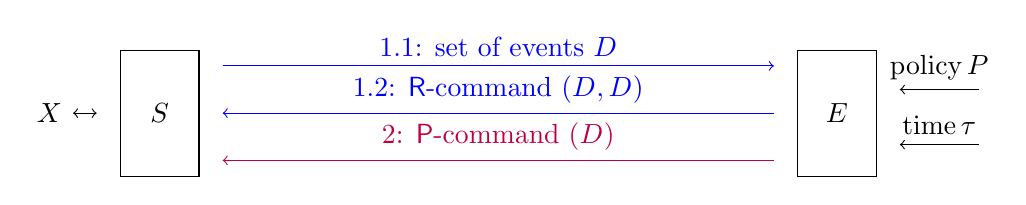
\begin{tikzpicture}
            \node at (-3.7,0.2) {$X$};
            \draw (-2.8,-0.6) rectangle (-1.8,1);
            \node at (-2.3,0.2) {$S$};
            \draw (5.8,-0.6) rectangle (6.8,1);
            \node at (6.3,0.2) {$E$};
            \draw[->,blue] (-1.5,0.8) to node[above] {1.1: set of events $D$} (5.5,0.8);
            \draw[<-,blue] (-1.5,0.2) to node[above]
                {1.2: $\mathsf{R}$-command
                $\RCom(D_{\Cau},D_{\Sup})$} (5.5,0.2);
            \draw[<-,purple] (-1.5,-0.4) to node[above]
                {2: $\mathsf{P}$-command $\PCom(D_{\Cau})$} (5.5,-0.4);
            \draw[<-] (7.1,0.5) to node[above] {policy\,$P$} (8.1,0.5);
            \draw[<->] (-3.4,0.2) to node[above] {} (-3.1,0.2);
            \draw[<-] (7.1,-0.2) to node[above] {time\,$\tau$} (8.1,-0.2);
        \end{tikzpicture}
    \end{center}
    \vspace{-1.5em}
    \caption{Proactive real-time first-order enforcement system model \cite[Figure 2]{whyenf}}
    \label{fig:system-model}
\end{figure}

We consider the system model of Hublet et. al \cite{whyenf} which is shown
in Figure \ref{fig:system-model}.
The system (under scrutiny) $S$ runs in some environment $X$.
The environment $X$ is not under the control of the enforcer $E$.
The enforcer $E$ must ensure that the system $S$ complies with some
policy $P$. To this end the enforcer is given two main ways of interaction
with the system. First, it can react to observable events happening in the system
via issuing $\mathsf{R}$-commands (reactively) by causing events of its own
and/or suppressing events before they are visible to the environment.
And second, the enforcer can issue $\mathsf{P}$-commands (proactively)
by causing certain events at some time-stamp $\tau$.

% TODO: elaborate and reformulate enforcement model

In the following the event names of events in sets denoted by
$D_\Cau$ are all assumed to be in $\Events_{\Cau}$ and
$D_\Sup$ are all assumed to be in $\Events_{\Sup}$.
The next three definitions reintroduce the three types of commands
used by Hublet et al. \cite{whyenf}.
\begin{definition}
    \label{def:enf-r-cmd}
    An \emph{R-Command} has the form
    $\RCom\left(D_{\Cau}, D_{\Sup}\right)$.
    This command is a reaction of the enforcer to some set of events $D$,
    that the system sent to the enforcer.
    The trace of the enforced system will contain the set
    $D_{\Cau} \cup \left(D \setminus D_{\Sup} \right)$ of events.
\end{definition}

\begin{definition}
    \label{def:enf-p-cmd}
    A \emph{P-Command} has the form
    $\PCom \left( D_{\Cau} \right)$.
    This command can be proactively issued by the enforcer before any
    clock tick to issue the set of events $D_{\Cau}$.
\end{definition}

\begin{definition}
    \label{def:enf-no-cmd}
    \emph{No-Command} has the form $\NCom$ and indicates that the enforcer takes
    no action.
\end{definition}

\begin{definition}
    The set of all commands is $\EnfCommands$.
\end{definition}

This leads us to Hublet et al.'s \cite{whyenf, whyenf-2} definition of a proactive enforcer.
\begin{definition}
    \label{def:enforcer-triple}
    An \emph{Enforcer} $\Enforcer$ is a triple
    $\left(\EnfStates, s_0, \EnfFun \right)$, where $\EnfStates$ is a set of 
    enforcer states
    $s_0 \in \EnfStates$ is an initial enforcer state and
    $\EnfFun : \Traces_f \times \EnfStates
    \times \Nat \times \left( \Databases \cup \left\{ \tick \right\} \right)
    \to \EnfCommands \times \EnfStates$
    is a computable update function such that the following two
    conditions hold
    \begin{enumerate}
        \item 
            $ \forall \sigma \in \Traces_f, \tau \in \Nat,
            % D \neq \tick,
            D \in \Databases,
            s \in \EnfStates.~
            \exists D_\Cau \in \Databases_\Cau, D_\Sup \in \Databases_\Sup,
            s' \in \EnfStates.$
        \begin{equation*}
            \mu(\sigma,s,\tau, D)
            = (\RCom(D_\Cau,D_\Sup), s') \wedge D_\Cau \subseteq D
        \end{equation*}
        
        \item
            $\forall \sigma \in \Traces_f, s \in \EnfStates, \tau \in \Nat.~
            \exists D_\Cau \in \Databases_\Cau, s' \in \EnfStates.$
            \begin{equation*}
                \mu(\sigma,s,\tau,\tick)
                \in \{(\PCom(D_\Cau), s'), (\NCom,s')\}
            \end{equation*}
    \end{enumerate}
\end{definition}
Hublet et al. \cite{whyenf-2} define an enforced trace algorithmically via
Algorithm~\ref{alg:loop}.

\begin{definition}
    \label{def:enforced-trace}
    For any $\sigma \in \Traces$ and enforcer  $\Enforcer=(\EnfStates,s_0,\mu)$, the
    \emph{enforced trace} $\Enforcer(\sigma)$ is defined co-recursively in
    Algorithm~\ref{alg:loop}.
    \begin{algorithm}[t]
        \begin{algorithmic}[1]
            \State $\run(s,\sigma,\sigma',\tau)=$~\Case\;$\sigma'$ \OOf
            \State $\mid \varepsilon \Rightarrow \varepsilon$
            \State $\mid(\tau', D) \cdot \sigma''$ \When\;$\tau' > \tau \Rightarrow$
            \Let\;$(o,s') = \mu(\sigma,s,\tau,\mathsf{tick})$ \IIn{}
            \State \quad \Case\;$o$ \OOf~$\mid\PCom(D_\Cau) \Rightarrow (\tau,D_\Cau) \cdot
                \run(s',\sigma\cdot (\tau, D_\Cau),\sigma',\tau+1)$
            \State \qquad\qquad\quad~$\mid\NCom \Rightarrow \run(s',\sigma,\sigma',\tau+1)$
            \State  $\mid(\tau', D) \cdot \sigma''$ \When\;$\tau' = \tau \Rightarrow$
            \Let\;$(o,s') = \mu(\sigma,s,\tau,D); D' = (D \setminus D_\Sup) \cup D_\Cau)$ \IIn
            \State \quad \Case\;$o$ \OOf ~$\mid \RCom(D_\Cau,D_\Sup)
                \Rightarrow (\tau, D') \cdot \run(s',\sigma \cdot (\tau, D'),\sigma'',\tau+1)$
            \State $\Enforcer(\sigma)=
                \run(s_0,\emptytrace,\sigma,\Ternaryop{\sigma=\emptytrace}{0}{\fts(\sigma)})$
        \end{algorithmic}
    \caption{Enforced trace\label{alg:loop} \cite[Fig. 2]{whyenf-2}}
    \vspace{-.6ex}
    \end{algorithm}
\end{definition}
In Definition \ref{def:enforced-trace} the trace $\sigma$ corresponds
to a system's behavior if it was running completely without an enforcer.
The enforced trace then represents the systems behavior combined with
those of the enforcer.
\begin{definition}
    \label{def:enf-sound-property}
    An enforcer $\Enforcer$ is \emph{sound} with respect to some property $P$, iff
    for any trace $\sigma \in \Traces_\omega$, $\Enforcer(\sigma) \in P$.
\end{definition}
\begin{definition}
    \label{def:enf-sound-policy}
    An enforcer $\Enforcer$ is \emph{sound} with respect to some policy $\phi$, iff
    it is sound for the language $\Language(\phi)$.
\end{definition}
Soundness allows us to describe and capture the behavior of an enforcer.

\begin{definition}
    \label{def:enf-transparent-property}
    An enforcer $\Enforcer = \left( \EnfStates, s_0, \EnfFun \right)$ is transparent
    with respect to some property $P$ iff for all $\sigma \in P$,
    $\Enforcer(\sigma) = \sigma$.
\end{definition}
\begin{definition}
    \label{def:enf-transparent-policy}
    An enforcer $\Enforcer = \left( \EnfStates, s_0, \EnfFun \right)$ is transparent
    with respect to some policy $\phi$ iff it is transparent for
    the language $\Language(\phi)$.
\end{definition}
Transparency means that an enforcer will not alter a trace that is already
compliant with some policy or property.
A property or policy is said to be \emph{(transparently) enforceable} if there
exists a (transparent) sound enforcer for the policy or property.


%%%%%%%%%%%%%%%%%%%%%%%%%%%%%%%%%%%%%%%%%%%%%%%%%%%%%%%%%%%%%%%%%%%%%%%%%%%%%%%%
\subsection{Enforceable MFOTL}
\label{subsection:emfotl}
% Hublet et al. \cite{whyenf} introduces a subset of MFOTL called Enforceable MFOTL,
% where every event gets marked with some capability which indicates the levels of power
% an enforcer has over an event.
Capabilities are an integral part of the proactive enforcement
approach introduced by Hublet et. al \cite{whyenf}.
Under this approach an enforcer can have different capabilities, or ways of interacting
with events emitted by a given system under scrutiny (SuS).
In Hublet et. al the set of capabilities consists of observable ($\Obs$),
suppressable ($\Sup$), causable ($\Cau$),
and suppressable-causable ($\Cau \Sup$).
Hublet et. al \cite{lex} expands this expands this system of capabilities, specifically it
makes the existence of events that may not (always) be externally visible explicit.
Under both notions a capability function $\kappa : \Events \to \Capabilities$ is used
to assign a capability to all events with some event name $e \in \Events$.
Also in both contexts, capabilities form a (semi)-lattice $(\Capabilities, \capleq)$.
% We write Sup as a shorthand for Suppressable and Cau as a shorthand for Causable.

% TODO: insert WhyEnf and Lex/CRE capability lattices

\begin{figure}
    
    \centering
    \begin{tikzpicture}
        % \node[text depth=0.1cm] (itl) at (1,1) {\texttt{internal}};
        \node[text depth=0.1cm] (cau_sup) at (1,0) {$\Cau \Sup$};
        
        \node[text depth=0.1cm] (cau_obs) at (-1,-1) {$\Cau \Obs$};
        \node[text depth=0.1cm] (sup) at (3,-1) {$\Sup$};
        
        \node[text depth=0.1cm] (obs) at (1,-2) {$\Obs$};
        \node[text depth=0.1cm] (cau) at (-3,-2) {$\Cau$};
        
        \node[text depth=0.1cm] (bot) at (-1,-3) {$\bot$};
        % \draw[->, dashed] (cau_sup) -- (itl);
        \draw[->] (sup) -- (cau_sup);
        \draw[->] (cau_obs) -- (cau_sup);
        \draw[->] (cau) -- (cau_obs);
        \draw[->] (obs) -- (cau_obs);
        \draw[->] (obs) -- (sup);
        \draw[->] (bot) -- (obs);
        \draw[->] (bot) -- (cau);
    \end{tikzpicture}
    % \vspace{-2em}
    \caption{The \emph{Capability Lattice} $(\Capabilities, \capleq)$
    \label{fig:capability-lattice}}
\end{figure}

\begin{definition}
    \label{def:cau-events}
    The subset of \emph{Causable Events}
    $$
    \Events_{\Cau} =
    \left\lbrace e \mid \Cau \capleq \kappa(e) \right\rbrace
    $$
    consists of all event names which can be caused by the enforcer,
    i.e. which have a capability of at least $\Cau$.
\end{definition}

\begin{definition}
    \label{def:sup-events}
    The subset of \emph{Suppressable Events}
    $$
    \Events_{\Sup} =
    \left\lbrace e \mid \Sup \capleq \kappa(e) \right\rbrace
    $$
    consists of all event names which can be suppressed by the enforcer, 
    i.e. which have a capability of at least $\Sup$.
\end{definition}

\begin{definition}
    \label{def:cau-databases}
    The set of \emph{Causable Databases} $\Databases_\Cau$ contains all
    sets of events that are at least causable.
    $$
        \Databases_\Cau =
        \left\{
        D \in \Databases \mid
        \forall e\left( \bar{t} \right) \in D. \ e \in \Events_\Cau
        \right\}
    $$
\end{definition}

\begin{definition}
    \label{def:sup-databases}
    The set of \emph{Suppressable Databases} $\Databases_\Sup$ contains all sets
    of events that are at least suppressable.
    $$
        \Databases_\Sup =
        \left\{
        D \in \Databases \mid
        \forall e\left( \bar{t} \right) \in D. \ e \in \Events_\Sup
        \right\}
    $$
\end{definition}

On the basis of capabilities
Hublet, Lima et al. \cite{whyenf, whyenf-2} introduce a subset of
MFOTL formulae that is enforceable.
The typing rules for this subset are shown in Figure \ref{fig:emfotl-typing-rules}.
These rules rely on the concept of past-guardedness, specifically for the
suppressability of existential quantifiers.
Past-guardedness means that all possible valuations of a variable in
the past are known.
The rules for past-guardedness are shown in Figure \ref{fig:past-guardedness}.

The signature $\Sigma$ of Example \ref{ex:signature} could be extended
with the following capabilities:
\begin{align*}
    &\kappa(\mathsf{sendEmail}) &= \Cau \Sup \\
    &\kappa(\mathsf{giveEmailConsent}) &= \Obs \\
    &\kappa(\mathsf{revokeEmailConsent}) &= \Obs.
\end{align*}
These capabilities capture, that an enforcer can both send and
prevent the sending of emails, but it cannot change the
consent given or revoked by a user.

\begin{figure}
    \begin{gather*}
        % https://tex.stackexchange.com/a/517660/282429 to suppress syntax errors caused by $-signs inside of gather environments in overleaf
        \prftree[r]
            %%begin novalidate
            {$\Events^+_\PG$}
            %%end novalidate
            {\gamma \vdash e(\dots, x, \dots) : \PG_E(x)^+}
        \quad
        \prftree[r]
            %%begin novalidate
            {$\neg_\PG$}
            %%end novalidate
            {\gamma \vdash \phi : \PG_E(x)^{\neg p}}
            {\gamma \vdash \neg \phi : \PG_E(x)^p}
        \\
        \prftree[r]
            %%begin novalidate
            {$\exists_\PG$}
            %%end novalidate
            {x \neq z}
            {\gamma \vdash \phi : \PG_E(z)^p}
            {\gamma \vdash \exists x .~ \phi : \PG_E(z)^p}
        \quad
        \prftree[r]
            %%begin novalidate
            {$\wedge_\PG^{\Left+}$}
            %%end novalidate
            {\gamma \vdash \phi : \PG_E(x)^+}
            {\gamma \vdash \phi \wedge \psi : \PG_E(x)^+}
            \\
        \prftree[r]
            %%begin novalidate
            {$\wedge_\PG^{\Right+}$}
            %%end novalidate
            {\gamma \vdash \psi : \PG_E(x)^+}
            {\gamma \vdash \phi \wedge \psi : \PG_E(x)^+}
            \quad
        \prftree[r]
            %%begin novalidate
            {$\wedge_\PG^-$}
            %%end novalidate
            {\gamma \vdash \phi : \PG_E(x)^-}
            {\gamma \vdash \psi : \PG_E(x)^-}
            {\gamma \vdash \phi \wedge \psi : \PG_E(x)^-}
            \\
        \prftree[r]
            %%begin novalidate
            {$\Since_\PG^{\Left+}$}
            %%end novalidate
            {0 \notin I}
            {\gamma \vdash \phi : \PG_E(x)^+}
            {\gamma \vdash \phi \Since_I \psi : \PG_E(x)^+}
            \quad
        \prftree[r]
            %%begin novalidate
            {$\Since_\PG^{\Right+}$}
            %%end novalidate
            {\gamma \vdash \psi : \PG_E(x)^+}
            {\gamma \vdash \phi \Since_I \psi : \PG_E(x)^+}
            \\
        \prftree[r]
            %%begin novalidate
            {$\Since_\PG^-$}
            %%end novalidate
            {0 \in I}
            {\gamma \vdash \psi : \PG_E(x)^-}
            {\gamma \vdash \phi \Since_I \psi : \PG_E(x)^-}
            \quad
        \prftree[r]
            %%begin novalidate
            {$\UUntil_\PG^{\Left+}$}
            %%end novalidate
            {0 \notin I}
            {\gamma \vdash \phi : \PG_E(x)^+}
            {\gamma \vdash \phi \UUntil_I \psi : \PG_E(x)^+}
            \\
        \prftree[r]
            %%begin novalidate
            {$\UUntil_\PG^{\LeftRight+}$}
            %%end novalidate
            {\gamma \vdash \phi : \PG_E(x)^+}
            {\gamma \vdash \psi : \PG_E(x)^+}
            {\gamma \vdash \phi \UUntil_I \psi : \PG(_Ex)^+}
            \quad
        \prftree[r]
            %%begin novalidate
            {$\UUntil_\PG^-$}
            %%end novalidate
            {0 \in I}
            {\gamma \vdash \psi : \PG_E(x)^-}
            {\gamma \vdash \phi \UUntil_I \psi : \PG_E(x)^-}
            \\
        \prftree[r]
            %%begin novalidate
            {$\Prev_\PG^+$}
            %%end novalidate
            {\gamma \vdash \phi : \PG_E(x)^+}
            {\gamma \vdash \Prev_I \phi : \PG_E(x)^+}
        \qquad
        \prftree[r]
            %%begin novalidate
            {$\gamma_\PG$}
            %%end novalidate
            {\gamma((e,i))=E}
            {\gamma \vdash e(x_1,\dots,x_i=x,\dots,x_k) : \PG_E^p(x)}
        \\
        \prftree[r]
            %%begin novalidate
            {$\mathsf{let}_\PG$}
            %%end novalidate
            {\forall i.~\gamma \vdash \phi_1 :\PG^p_{E_i}(x_i)}
            {\gamma, (e,1) : E_1,\dots, (e,k):E_k \vdash \phi_2 : \PG^p_{E}(x)}
            {\gamma \vdash \LLet{e(x_1,\dots,x_k)}{\phi_1}{\phi_2}:\PG^p_{E}(x)}
    \end{gather*}
    \vspace{-2em}
    \caption{Past-Guardedness Rules \label{fig:past-guardedness}}
\end{figure}

\begin{figure}
    \begin{gather*}
        % https://tex.stackexchange.com/a/517660/282429 to suppress syntax errors caused by $-signs inside of gather environments in overleaf
        \prftree[r]
            %%begin novalidate
            {$\top^\Cau$}
            %%end novalidate
            {\Gamma \vdash \top : \Cau}
            \quad
        \prftree[r]
            %%begin novalidate
            {$\bot^\Sup$}
            %%end novalidate
            {\Gamma \vdash \bot : \Sup}
            \quad
        \prftree[r]
            %%begin novalidate
            {$\Events^\Cau$}
            %%end novalidate
            {e \in \Cau}
            {\Gamma(e) = \Cau}
            {\Gamma \vdash  e(t_1,\dots,t_k) : \Cau}
            \\
        \prftree[r]
            %%begin novalidate
            {$\Events^\Sup$}
            %%end novalidate
            {e \in \Sup}
            {\Gamma(e) = \Sup}
            {\Gamma \vdash  e(t_1,\dots,t_k) : \Sup}
            \quad
        \prftree[r]
            %%begin novalidate
            {$\neg^\Cau$}
            %%end novalidate
            {\Gamma \vdash \phi : \Sup}
            {\Gamma \vdash \neg \phi : \Cau}
            \quad
        \prftree[r]
            %%begin novalidate
            {$\neg^\Sup$}
            %%end novalidate
            {\Gamma \vdash \phi : \Cau}
            {\Gamma \vdash \neg \phi : \Sup}
            \\
        \prftree[r]
            %%begin novalidate
            {$\exists^\Cau$}
            %%end novalidate
            {\Gamma \vdash \phi : \Cau}
            {\Gamma \vdash \exists x.~\phi : \Cau}
            \quad
        \prftree[r]
            %%begin novalidate
            {$\exists^\Sup$}
            %%end novalidate
            {\Gamma \vdash \phi : \Sup}
            {\vdash \phi : \PG(x)^+}
            {\Gamma \vdash \exists x.~\phi : \Sup}
            \quad
        \prftree[r]
            %%begin novalidate
            {$\wedge^\Cau$}
            %%end novalidate
            {\Gamma \vdash \phi : \Cau}
            {\Gamma \vdash \psi : \Cau}
            {\Gamma \vdash \phi \wedge \psi : \Cau}
            \\
        \prftree[r]
            %%begin novalidate
            {$\wedge^{\Sup\Left}$}
            %%end novalidate
            {\Gamma \vdash \phi : \Sup}
            {\Gamma \vdash \phi \wedge \psi : \Sup}
            \quad
        \prftree[r]
            %%begin novalidate
            {$\wedge^{\Sup\Right}$}
            %%end novalidate
            {\Gamma\vdash \psi : \Sup}
            {\Gamma \vdash \phi \wedge \psi : \Sup}
            \quad
        \prftree[r]
            %%begin novalidate
            {$\Since^\Cau$}
            %%end novalidate
            {0 \in I}
            {\Gamma \vdash \psi : \Cau}
            {\Gamma \vdash \phi \Since_I \psi : \Cau}
            \\
        \prftree[r]
            %%begin novalidate
            {$\Since^{\Sup\Left}$}
            %%end novalidate
            {0 \notin I}
            {\Gamma \vdash \phi : \Sup}
            {\Gamma \vdash \phi \Since_{I} \psi : \Sup}
            \quad
        \prftree[r]
            %%begin novalidate
            {$\Since^{\Sup\LeftRight}$}
            %%end novalidate
            {0 \in I}
            {\Gamma \vdash \phi : \Sup}
            {\Gamma \vdash \psi : \Sup}
            {\Gamma \vdash \phi \Since_I \psi : \Sup}
            \\
        \prftree[r]
            %%begin novalidate
            {$\UUntil^\Sup$}
            %%end novalidate
            {\Gamma \vdash \psi : \Sup}
            {\Gamma \vdash \phi \UUntil_I \psi : \Sup}
            \quad
        \prftree[r]
            %%begin novalidate
            {$\UUntil^{\Cau\Right}$}
            %%end novalidate
            {b \neq \infty}
            {\Gamma \vdash \psi : \Cau}
            {\Gamma \vdash \phi \UUntil_{[0,b]} \psi : \Cau}
            \\
        \prftree[r]
            %%begin novalidate
            {$\UUntil^{\Cau\LeftRight}$}
            %%end novalidate
            {b \neq \infty}
            {\Gamma\vdash \phi : \Cau}
            {\Gamma \vdash \psi : \Cau}
            {\Gamma \vdash \phi \UUntil_{[a,b]} \psi : \Cau}
            \quad
        \prftree[r]
            %%begin novalidate
            {$\Next^\Cau$}
            %%end novalidate
            {\Gamma \vdash \phi : \Cau}
            {b > 0}
            {\Gamma \vdash \Next_{[0,b)} \phi : \Cau}
            \\
        \prftree[r]
            %%begin novalidate
            {$\Next^\Sup$}
            %%end novalidate
            {\Gamma \vdash \phi : \Sup}
            {\Gamma \vdash \Next_I \phi : \Sup}
        \qquad
        \prftree[r]
            %%begin novalidate
            {$\mathsf{let}$}
            %%end novalidate
            {\Gamma \vdash \phi_1 : \tau_1}
            {\Gamma, e : \tau_1 \vdash \phi_2 : \tau_2}
            {\Gamma \vdash \LLet{e(\overline{t})}{\phi_1}{\phi_2} : \tau_2}
    \end{gather*}
    \vspace{-2em}
    \caption{EMFOTL Typing Rules \label{fig:emfotl-typing-rules}}
\end{figure}

% For enforcement under a condition as in Definition
% \ref{def:enf-sound-policy-under-condtion} we can add one additional
% typing rule to expand the fragment of enforceable MFOTL formulae.

% \begin{definition}
%     % TODO: is this needed? or ever referenced?
%     \label{def:emfotl-under-condition-additional-typing-rule}
%     Additional typing rule when enforcement is done under some condition
%     \begin{equation*}
%         \prftree[r]
%             % https://tex.stackexchange.com/a/517660/282429 to suppress syntax errors caused by $-signs inside of gather environments in overleaf
%             %%begin novalidate
%             {$\mathsf{C}^\Cau$}
%             %%end novalidate
%             {\psi \to \phi}
%             {\Gamma \vdash_\psi \phi : \Cau}
%     \end{equation*}
% \end{definition}

% To give some intuition for this rule, we can imagine an MFOTL formula $\phi$
% that is not causable (i.e. enforceable) under the general EMFOTL typing
% rules.
% If we make this formula $\phi$ now a condition (i.e. we assume it to be true),
% it does become "causable" by assumption.
% Now it is important that this is a very different notion of causability since
% it is not the enforcer that can cause a certain event, but rather it is
% a circumstance that is assumed to hold externally.
% % TODO: give a more concrete example
% % TODO: formulate enforcement under a condition/assumption more clearly
% The "condition"-subscript ($\psi$ in Definition
% \ref{def:emfotl-under-condition-additional-typing-rule}) can propagate through
% the rule in Figure \ref{fig:emfotl-typing-rules}.

%%%%%%%%%%%%%%%%%%%%%%%%%%%%%%%%%%%%%%%%%%%%%%%%%%%%%%%%%%%%%%%%%%%%%%%%%%%%%%%%
%                                                                              %
%%%%%%%%%%%%%%%%%%%%%%%%%%%%%%%%%%%%%%%%%%%%%%%%%%%%%%%%%%%%%%%%%%%%%%%%%%%%%%%%
\subsection{Constitutive, Regulative, and Exception Rules}
\label{section:cre-meta-logic}

%%%%%%%%%%%%%%%%%%%%%%%%%%%%%%%%%%%%%%%%%%%%%%%%%%%%%%%%%%%%%%%%%%%%%%%%%%%%%%%%
\subsection{Introduction}
\label{subsection:cre-meta-logic}
Hublet et. al \cite{lex} introduce a meta-logic based on
constitutive, regulative, and exception rules (CRE meta-logic).
The CRE meta-logic underpins the Lex programming language
and formalizes how a Lex specification would compiles
to an MFOTL formula.

\begin{definition}
    \label{def:cre-rule-labels}
    The \emph{set of rule labels} is denoted by $\RLabels$.
\end{definition}

\begin{definition}
    \label{def:cre-mfotl-signature}
    A \emph{CRE[MFOTL] Signature} is a quadruple of the following form
    $$
    \Sigma' = ( \Domain, 
    \Events \cup \Events',
    \Functions, \iota \cup \iota'
    ).
    $$
    Where $\Domain$ is a domain of values,
    $\Events$ is a set of external event names,
    $\Events'$ is a set of internal event names,
    $\Functions$ is a set of function names,
    $\iota: \Events \cup \Functions \to \Nat$ is an external arity funciton,
    and $\iota': \Events' \to \Nat$ is an internal arity function.
    $\Events$ and $\Events'$ are disjoint.
\end{definition}
CRE[MFOTL] signatures are very similar to MFOTL signatures, but include
the addition of internal events.
While it is useful to distinguish between internal and external events,
in CRE[MFOTL] and later in Lex, a CRE[MFOTL] signature can still be used
as an MFOTL signature.
Therefore the next definition deifnes the set of valid MFOTL
formulae over a CRE[MFOTL] signature.

% \begin{example}
%     \label{ex:cre-signature}
%     The MFOTL signature $\Sigma$ of Example \ref{ex:signature} can be
%     extended to a CRE[MFOTL] signature $\Sigma'$ by adding the following
%     internal event
%     \begin{align*}
%         \Events' = \{ &\mathsf{userPressedConsentButton}, \\
%                       & \mathsf{userPressedRevokeButton}, \\
%                       & \mathsf{userGaveConsentByEail}, \\
%                       & \mathsf{userRevokedConsentByEmail}
%                    \}
%     \end{align*}
%     and extending the arity function $\iota'$ to
%     \begin{align*}
%         \iota'(\mathsf{userPressedConsentButton}) &= 2 \\
%         \iota'(\mathsf{userPressedRevokeButton}) &= 2 \\
%         \iota'(\mathsf{userGaveConsentByEail}) &= 2 \\
%         \iota'(\mathsf{userRevokedConsentByEmail}) &= 2.
%     \end{align*}
%     Then $\Sigma' = (\Domain, \Events \cup \Events', \Functions, \iota \cup \iota')$    
%     is a CRE[MFOTL] signature, where $\Domain, \Events, \Functions, \iota$
%     are the same as in Example \ref{ex:signature}.
% \end{example}

\begin{definition}
    \label{def:set-of-mfotl-formulae}
    The \emph{set of all MFOTL formulae} over a CRE[MFOTL] signature
    $\Sigma'$ is denoted by $\formulae$.
\end{definition}

Next we recall constitutive, regulative, and exception rules
\cite[Section 3.1]{lex}.

\begin{table}
    \centering
    \begin{tabular}{|r|l|l|}
        \hline
        \textbf{Rule Type}
        & \textbf{Syntax}
        & \textbf{Meaning} \\ 
        \hline
        Constitutive
            & $r: \phi \Rightarrow e(\bar{x})$
            & "$\phi$ counts as $e(\bar{x})$"
            \\
        \hline
        Regulative
            & $r: \phi \Rightarrow \psi$
            & "if $\phi$ holds, then $\psi$ must hold"
            \\
        \hline
        Exception
            & $r: \phi \Rightarrow \exc(s)$
            & "if $\phi$ holds, then rule $s$ shall not apply"
            \\
        \hline
    \end{tabular}
    \caption{CRE[MFOTL] Rule Types \label{tab:cre-rule-types}}
\end{table}

\begin{definition}
    \label{def:cre-rules}
    Let $r,s \in \RLabels$, $\phi, \psi \in \formulae$, $e \in \Events'$,
    $x_1, \dots, x_{\iota'(e)} \in \Domain$,
    and $\bar{x} = (x_1, \dots, x_{\iota'(e)})$.
    Table \ref{tab:cre-rule-types} gives an
    overview over the three rule types, their syntax, and
    their meaning.
\end{definition}

\begin{definition}
    \label{def:cre-policy}
    A \emph{CRE Policy} is a triple $\Phi = \left(C, R, E\right)$
    where $C$ is a set of constitutive rules, $R$ is a set of regulative
    rules, and $E$ is a set of exception rules such that
    every rule in $C \cup R \cup E$ has a unique label.
\end{definition}

\begin{figure}
    \begin{align*}
        [\textsc{con}] &&
            \gamma &\vDash^\Phi p &&
            \text{iff } r:\phi \Rightarrow p \in C
            \text{ and }\gamma \vDash^\Phi \phi \wedge \neg \exc(r) \\
        [\textsc{reg}] &&
            \gamma &\vDash^\Phi \comply(r) &&
            \text{iff } r:\phi \Rightarrow \psi \in R
            \text{ and }\gamma \vDash^\Phi (\phi \to \psi) \vee \exc(r)\\
        [\textsc{exc}] &&
            \gamma &\vDash^\Phi \exc(s) &&
            \text{iff } r:\phi \Rightarrow \exc(s) \in E
            \text{ and }\gamma \vDash^\Phi \phi \wedge \neg \exc(r)
    \end{align*}
    \vspace{-2em}
    \caption{Semantics of CRE for a fixed structure\label{fig:cre-semantics} \cite[Figure 5]{lex}}
\end{figure}

Figure \ref{fig:cre-semantics} defines the semantics of the CRE[MFOTL] logic.
The semantics expand the logic of $\formulae$ the CRE[MFOTL] logic
is captured by $\gamma \vDash \phi$.
These semantics can be expanded to define compliance for an entire CRE-policy as followed.
\begin{definition}
    \label{cre-compliance}
    A CRE-policy $\Phi = \left(C,R,R \right)$ is complied with ($\gamma \vDash \Phi$), if
    all its regulative rules are complied with, which is captured in the rule:
    \begin{equation*}
        \prftree[r]{CRE-Compliance}
            {\forall r: \phi \Rightarrow \psi \in R.\ \comply(r)}
            {\gamma \vDash \Phi}
    \end{equation*}
\end{definition}

\begin{definition}
    \label{def:cre-specification}
    A \emph{CRE Specification} 
    $\Specification = \left(\Sigma, \phi, \kappa \right)$
    is a triple consisting of some signature
    $\Sigma = \left(\Domain, \Events, \Functions, \iota \right)$,
    some CRE policy
    $\Phi = \left(C, R, E\right)$,
    and a capability-mapping $\kappa$.
\end{definition}

Analogous to EMFOTL, Hublet et al. \cite{lex} define enforceable
CRE (ECRE)
via the typing rules in Figure \ref{fig:ecre-typing-rules}

\begin{example}
    \label{ex:cre-policy}
    The MFOTL policy $\Phi$ of Example \ref{ex:mfotl-formula}
    could be captured in the following CRE[MFOTL] policy:

    \begin{align*}
        C &= \{
            r :
            &&\mathsf{sendEmail}(\mathsf{user}, \text{"marketing"})
            \Rightarrow \\
            &&&(\Once_{[0,\infty)} 
                \mathsf{giveEmailConsent}(\mathsf{user}, \text{"marketing"}) \\
                &&&\quad \wedge
                ((\neg
                \mathsf{revokeEmailConsent}(\mathsf{user}, \text{"marketing"})) \\
                &&& \qquad \Since_{[0,\infty)}
                \mathsf{giveEmailConsent}(\mathsf{user}, \text{"marketing"})))
        \} \\
        R &= \emptyset \\
        E &= \emptyset
    \end{align*}
    $\Phi := (C,R,E)$ is a CRE[MFOTL] policy consisting of a single
    regulative rule $r$.
\end{example}

\begin{figure}
    % https://tex.stackexchange.com/a/517660/282429 to suppress syntax errors caused by $-signs inside of gather environments in overleaf
    \begin{gather*}
        \prftree[r]{\textsc{regI}}
            {r : \phi \Rightarrow \psi \in R}
            {\overline{x}=\fv(\phi) \cup \fv(\psi)}
            {\Gamma \vdash^\Phi \Always (\forall \overline{x}.~\phi \rightarrow \psi) : \Cau}
            {\Gamma \vdash^\Phi \comply(r) : \Cau} \\
        \prftree[r]{\textsc{regE}}
            {r : \phi \Rightarrow \psi \in R}
            {\overline{x}=\fv(\phi) \cup \fv(\psi)} 
            {\Gamma \vdash^\Phi \Always
                (\forall \overline{x}.~\phi \land \neg \psi \rightarrow \exc(r)) : \Cau}
            { \Gamma \vdash^\Phi \comply(r) : \Cau} \\
        \prftree[r]{$\textsc{exc}^\Cau$}
            {r : \phi \Rightarrow \exc(s) \in E}
            {\Gamma \vdash^\Phi \phi : \Cau}
            {\Gamma \vdash^\Phi \exc(r) : \Sup}
            {\Gamma \vdash^\Phi \exc(s) : \Cau} \\
        \prftree[r]{$\textsc{exc}^\Sup$}
            {\forall r : \phi \Rightarrow \exc(s) \in E.~
                (\Gamma \vdash^\Phi \phi : \Sup~\mathbf{or}~\Gamma \vdash^\Phi \exc(r) : \Cau)}
            {\Gamma \vdash^\Phi \exc(s) : \Sup} \\
        \prftree[r]{$\textsc{con}^\Cau$}
            {r : \phi \Rightarrow p \in C}
            {\Gamma \vdash^\Phi \phi : \Cau}
            {\Gamma \vdash^\Phi \exc(r) : \Sup}
            {\Gamma \vdash^\Phi p : \Cau} \\
        \prftree[r]{$\textsc{con}^\Sup$}
            {\forall r : \phi \Rightarrow p \in C.~
                (\Gamma \vdash^\Phi \phi : \Sup~\mathbf{or}~\Gamma \vdash^\Phi \exc(r) : \Cau)}
            {\Gamma \vdash^\Phi p : \Sup}
    \end{gather*}
    \vspace{-2em}
    \caption{Typing rules for ECRE[MFOTL] policies\label{fig:ecre-typing-rules} \cite[Figure 6]{lex}}
\end{figure}

%%%%%%%%%%%%%%%%%%%%%%%%%%%%%%%%%%%%%%%%%%%%%%%%%%%%%%%%%%%%%%%%%%%%%%%%%%%%%%%%
%                                                                              %
%%%%%%%%%%%%%%%%%%%%%%%%%%%%%%%%%%%%%%%%%%%%%%%%%%%%%%%%%%%%%%%%%%%%%%%%%%%%%%%%
\subsection{Compilation of CRE[MFOTL] to MFOTL}
\label{section:cre-compilation}
This section recalls the compilation algorithm of CRE[MFOTL] to Lex
as it is introduced in Hublet et al. \cite[Section 3.2]{lex}.
Hublet et al. \cite{lex} define the following dependency relation between
constitutive and exception rules analogous to
Merigoux et al. \cite[Section 4.1]{merigoux_catala_2021}.

\begin{definition}
    \label{def:cre-dependency-relation}
    For a CRE[MFOTL] Policy $\Phi := (C,R,E)$ let $r,s \in C \cup E$.
    $r \triangleright_\Phi s$ (read as "s depends on r")
    iff either $r:\phi \Rightarrow p \in C$ and $p$ occurs in the
    left-hand side of the rule $s$, or
    $r:\phi \Rightarrow \exc(s) \in E$.
\end{definition}

A policy $(C,R,E)$ is called \emph{acyclic} iff there do not exist two 
rules $r,s \in C \cup E$ such that $r \triangleright_\Phi s$,
and $s \triangleright_\Phi r$ and also that there is no single rule $r \in C \cup E$
that is self-referential (i.e. $r \triangleright_\Phi r$).
The compilation of CRE[MFOTL] to MFOTL is defined by Algorithm 
\ref{alg:compilation} and Algorithm \ref{alg:collect}.

\begin{algorithm}
  \caption{CRE[MFOTL] to MFOTL compilation
  \label{alg:compilation}\cite[Algorithm 1]{lex} }
  \begin{algorithmic}[1]
    \State \IInput $\mathcal{S}=(\Sigma,\Phi,\kappa)$ with $\Sigma = (\Domain, \Events, \Functions, \iota)$ and acyclic CRE[MFOTL] policy $\Phi=(C,R,E)$
    \State $\Events_E \gets \{ e_s \mid r: \phi \Rightarrow \exc(s) \in E \}$\label{alg:events_e}
    \State $R' \gets \{ r: \phi \land \neg e_r \Rightarrow \psi \mid r: \phi \Rightarrow \psi \in R, e_r \in \Events_E \} \cup \{ r: \phi \Rightarrow \psi \mid r: \phi \Rightarrow \psi \in R, e_r \notin \Events_E \}$\label{alg:r_prime}
    \State $C_E \gets \{ r: \phi \Rightarrow e_s \mid r: \phi \Rightarrow \exc(s) \in E \}$\label{alg:c_e}
    \State $\Events_0 \gets \{ p \mid p \not\in \Events \land e \text{ occurs in } C \cup R \cup E  \} \setminus \{ p \mid r: \phi \Rightarrow p \in C\}$\label{alg:events_0}
    \State $C_0 \gets \{ z_p: \bot \Rightarrow p \mid p \in \Events_0 \}$\label{alg:c_0}
    \State $C' \gets C \cup C_E \cup C_0$\label{alg:c_prime_1}
    \State $C' \gets \{ r: \phi \land \neg e_r \Rightarrow p \mid r: \phi \Rightarrow p \in C', e_r \in \Events_E \} \cup \{ r: \phi \Rightarrow p \mid r: \phi \Rightarrow p \in R, e_r \notin \Events_E \}$\label{alg:c_prime_2}
    \State $[(\phi_1, p_1),\dots, (\phi_k, p_k)] \gets \textsf{\textsc{collect}}(\textsf{\textsc{topological\_sort}}_{\triangleright_\Phi}(C'))$\label{alg:collected}
    \State \textbf{for} $r : \phi \Rightarrow \psi \in R'$ \textbf{do} $\overline{x}_r \gets \mathsf{free\_variables}(\phi \rightarrow \psi)$ \textbf{endfor}
    \State $\phi \gets \LLet{p_1}{\phi_1}{\dots\LLet{p_k}{\phi_k}{\bigwedge_{r: \phi \Rightarrow \psi \in R'}(\Always(\forall \overline{x}_r.~ \phi \to \psi))}}$\label{alg:phi}
    \State \OOutput $\mathcal{S}'=(\Sigma',\phi,\kappa)$ where $\Sigma' = (\Domain, \Events\setminus \{p_i \mid 1 \leq i \leq k\}, \Functions, \iota)$
\end{algorithmic}
\end{algorithm}

\begin{algorithm}
  \caption{Auxiliary function \textsc{\textsf{collect}}
  \label{alg:collect}\cite[Algorithm 2]{lex}}
  \begin{algorithmic}[1]
    \Function{\textsf{collect}}{$L$}
    \State\hspace{-1.25em}$P, L' \gets \emptyset, []$
    \State\hspace{-1.25em}\textbf{for }$r : \phi \Rightarrow p \in L$\textbf{ do}
    \State\hspace{-1em}\textbf{if } $p \notin P$ \textbf{ then } $(P, L') \gets (P \cup \{p\}, L' \cdot [(\bigvee_{r: \phi \Rightarrow p \in L} \phi, p)])$ \textbf{ endif}
    \State\hspace{-1.25em}\textbf{endfor}
    \State\hspace{-1.25em}\Return $L'$
    \EndFunction
  \end{algorithmic}
\end{algorithm}

%%%%%%%%%%%%%%%%%%%%%%%%%%%%%%%%%%%%%%%%%%%%%%%%%%%%%%%%%%%%%%%%%%%%%%%%%%%%%%%%
%                                                                              %
%%%%%%%%%%%%%%%%%%%%%%%%%%%%%%%%%%%%%%%%%%%%%%%%%%%%%%%%%%%%%%%%%%%%%%%%%%%%%%%%
\section{The Lex Programming Language}
\label{section:lex}
Hublet et al. \cite{lex} and Degelo \cite{semesterproject}
developed the Lex programming language based on CRE[MFOTL].
Lex is designed to formalize legal texts and maintain a high
readability, especially compared to pure MFOTL.
It achieves this readability by maintaining the general
structure of the underlying legal text.

%%%%%%%%%%%%%%%%%%%%%%%%%%%%%%%%%%%%%%%%%%%%%%%%%%%%%%%%%%%%%%%%%%%%%%%%%%%%%%%%
%                                                                              %
%%%%%%%%%%%%%%%%%%%%%%%%%%%%%%%%%%%%%%%%%%%%%%%%%%%%%%%%%%%%%%%%%%%%%%%%%%%%%%%%
\subsection{Lex Syntax}
\label{subsection:lex-syntax}

\begin{figure*}
    \begin{tabular}{|r|l|l|}
    \toprule
    \multirow{9}{*}
        {\Lex{}}
            &\kw{law}~$lbl$~[\stringkw{title}]
                &[$\tau$]~\kw{event}~$e$ \\
            &\kw{article}~$lbl$~[\stringkw{title}]
                &\qquad\triplestringkw{<docstring>} \\
            &\kw{paragraph}~$lbl$\dots
                &\qquad $x_1$ : $t_1$ \\
            &\kw{point}~$lbl$\dots
                &\qquad\dots \\
            &\dots
                &\qquad $x_k$ : $t_k$ \\
            &
                &$\tau::= \kw{observable}$ \\
            &\kw{type}~$t_1$~[\kw{is}~$t_2$]
                &\qquad$\mid\kw{suppressable}$ \\
            &\qquad\triplestringkw{<docstring>}
                &\qquad$\mid\kw{causable}~\mid\kw{internal}...$ \\
    \midrule
    \multirow{3}{*}
        {CRE[MFOTL]}
            &\multirow{3}{*}
                {n.a.}
                &$e \in \Events$ \\
            &
                &$\iota(e)=(t_1, \dots, t_k)$ \\
            &
                &$\kappa(e)=\Obs,\Sup,\Cau...$ \\
    \bottomrule
    \end{tabular}
    \vspace{1em}
    \begin{tabular}{|l|l|l|}
    \toprule
        \kw{rule}~$r$
            &\kw{rule}~$r$
            &\kw{rule}~$r$ \\
        \quad \kw{whenever}
            &\quad \kw{whenever}
            &\quad \kw{whenever} \\
        \qquad $\phi_1$
            &\qquad $\phi_1$
            &\qquad $\phi_1$ \\
        \qquad $\dots$
            &\qquad $\dots$
            &\qquad $\dots$ \\
        \qquad $\phi_k$
            &\qquad $\phi_k$
            &\qquad $\phi_k$ \\
        \quad \kw{constitute}
            &\quad \kw{oblige}
            &\quad \kw{except} \\
        \qquad $p_1$
            &\qquad $\psi_1$
            &\qquad $lbl_1$ \\
        \qquad $\dots$
            &\qquad $\dots$
            &\qquad $\dots$ \\
        \qquad $p_\ell$
            &\qquad $\psi_\ell$
            &\qquad $lbl_\ell$ \\
    \midrule
        % \multirow{3}{*}
        $r_1: \bigwedge\limits_{1 \leq i \leq k} \phi_i \Rightarrow p_1 \in C$
            & $r_1: \bigwedge\limits_{1 \leq i \leq k} \phi_i \Rightarrow \psi_1 \in R$
            & $r_1: \bigwedge\limits_{1 \leq i \leq k} \phi_i \Rightarrow \exc(s_1) \in E$ \\
        \dots
            & \dots
            & \dots\\
        $r_k: \bigwedge\limits_{1 \leq i \leq k} \phi_\ell\Rightarrow p_\ell \in C$
            & $r_k: \bigwedge\limits_{1 \leq i \leq k} \phi_\ell\Rightarrow \psi_\ell \in R$
            & $r_k: \bigwedge\limits_{1 \leq i \leq k} \phi_\ell\Rightarrow \exc(s_\ell) \in E$\\
    \bottomrule
    \end{tabular}
    \vspace{-1.8em}
    \caption{Correspondence between the \Lex{} and CRE[MFOTL] syntax
    \label{fig:lex-and-cre-correspondence}
    \cite[Figure 10]{lex}
    }
\end{figure*}

Lex has the following main types of statements:
\begin{itemize}
    \item \textbf{Section Labels}
        (keywords: \kw{law}, \kw{title}, \kw{chapter},
        \kw{section}, \kw{article}, \kw{paragraph},
        \kw{point}, \kw{subpoint})
        Section labels are used to represent the structure of
        the law.
        Section label statements have the form
        of a section keyword followed by a mandatory string
        identifier and an optional, more descriptive, string
        title (e.g. \kw{article} "1" "Preconditions").
        Section labels (together with optional rule identifiers)
        are the analog of rule labels in CRE[MFOTL].
        Section \ref{subsection:lex-section-labels} will go
        more in depth on section labels in Lex.
    \item \textbf{Type Declarations}
        (keyword: \kw{type})
        Type declarations map a type alias to a base type 
        (e.g. \kw{type} user \kw{is} string,
        \kw{type} age \kw{is} int).
        These type aliases are not represented in CRE[MFOTL].
    \item \textbf{Event Declarations}
        (keywords: \kw{event}, \kw{predicate})
        Event declarations declare event names and their arguments
        along with their types.
    \item \textbf{Function Declarations}
        (keyword: \kw{function})
        Function declarations are analogous to event declarations,
        but they define function names with their arguments and a
        return type.
    \item \textbf{Rule Definitions}
        (keyword: \kw{rule})
        Rule definitions are the core of the \Lex language.
        They define the constitutive, regulative, and exception
        rules like in CRE[MFOTL].
        \Lex rules are more verbose than those in CRE[MFOTL]
        and allow for the use of keywords in addition to symbols
        for temporal/logical operators
        (e.g. \graykw{ALWAYS} for $\Always$).
        A CRE[MFOTL] rule like $r: \phi \Rightarrow p \in C$
        becomse \kw{rule} \kw{whenever} $\phi$ \kw{constitute} $p$ in \Lex.
        After the \kw{rule} keyword, a rule can optionally
        be given a string identifier.
        Exception rules in \Lex make use of section labels and
        the optional rule identifiers to specify which rule(s)
        the apply to.
    \item \textbf{Import Statements}
        (keyword: \kw{import})
        Import statements are used to modularly split
        a \Lex specification into multiple files.
        "\kw{import} specification" imports the
        specification in the file "specification.lex".
\end{itemize}

Figure \ref{fig:lex-and-cre-correspondence}
shows the correspondence between Lex and CRE[MFOTL].

%%%%%%%%%%%%%%%%%%%%%%%%%%%%%%%%%%%%%%%%%%%%%%%%%%%%%%%%%%%%%%%%%%%%%%%%%%%%%%%%
%                                                                              %
%%%%%%%%%%%%%%%%%%%%%%%%%%%%%%%%%%%%%%%%%%%%%%%%%%%%%%%%%%%%%%%%%%%%%%%%%%%%%%%%
\subsection{Lex Section Labels}
\label{subsection:lex-section-labels}
The Lex language provides a fixed set of section label keywords:
\kw{law}, \kw{title}, \kw{chapter}, \kw{section},
\kw{article}, \kw{paragraph}, \kw{point}, \kw{subpoint}.
Not every law will have all of these hierarchical levels,
and besides \kw{law} and \kw{article} they are all optional.
If a law contains a hierarchical level that does not fit into
these predifined keywords, custom sub-levels can be defined
underneath one of the predifined ones
(e.g. \kw{article}[1] is a level below an article,
but above a paragraph; This has the consequence that \kw{article}
is implicitly equivalent to \kw{article}[0]).
As an example, a law might be the GDPR, which is further divided
into chapters and chapters then contain individual articles.
Another example would be the Swiss constitution as a law, which
is divided into titles.
While often times sections, titles, articles, etc. will be numbered,
in Lex they are refered to by strings.
This is due to the fact that no standard numbering scheme exists,
sometimes articles will contain letters like Article 1b, and other
times Roman numerals might be used.
One interesting aspect of laws across contexts is that
articles tend to be numbered continuously,
i.e. in the GDPR one doesn't need to know in which Chapter an
article is located, to uniquely refer to it.

References to other parts of a Lex specification can
always be made by stating all levels can always be made
by giving the full path consisting of all intermediate levels.
Due to the continuous (and thus unique) numbering of articles,
for sections below the \kw{article} level, it is not necessary to
include any levels between law and article.
Lex will also try to resolve references dynamically,
e.g. if \kw{article} "2" is used in \kw{article} "1", Lex
will attempt to resolve this reference inside the same \kw{law}.

%%%%%%%%%%%%%%%%%%%%%%%%%%%%%%%%%%%%%%%%%%%%%%%%%%%%%%%%%%%%%%%%%%%%%%%%%%%%%%%%
%                                                                              %
%%%%%%%%%%%%%%%%%%%%%%%%%%%%%%%%%%%%%%%%%%%%%%%%%%%%%%%%%%%%%%%%%%%%%%%%%%%%%%%%
\subsection{Lex - E-Mail Marketing Exmaple}
\label{subsection:lex-email-marketing-example}

This subsection will showcase the Lex language
on a hands on example.
Chapter \ref{chapter:methodology} will continue
this example to showcase how a Lex specification
can be refined.
The example is based on the 2002 ePrivacy Directive
of the European Union. % TODO: add some kind of source/link
Specifically we focus on Article 13 of the ePrivacy Directive.
This article regulates the use of electronic communication,
automated calls, fax, and e-mail for marketing purposes.

\begin{figure}
    % \hspace{-5mm}
    \begin{minipage}{\columnwidth}
    \begin{quote}
        \small \itshape
        Art. 13 ePrivacy Directive . \textbf{Unsolicited communications}

        \begin{enumerate}[1.]
            \item
            The use of automated calling systems without human
            intervention (automatic calling machines), facsimile machines
            (fax) or electronic mail for the purposes of direct marketing
            may only be allowed in respect of subscribers who have given
            their prior consent.
            \item
            Notwithstanding paragraph 1, where a natural or legal
            person obtains from its customers their electronic contact
            details for electronic mail, in the context of the sale of a
            product or a service, in accordance with Directive 95/46/EC,
            the same natural or legal person may use these electronic
            contact details for direct marketing of its own similar products
            or services provided that customers clearly and distinctly are
            given the opportunity to object, free of charge and in an easy
            manner, to such use of electronic contact details when they are
            collected and on the occasion of each message in case the
            customer has not initially refused such use.
            \item
            Member States shall take appropriate measures to ensure
            that [...] unsolicited communications for purposes
            of direct marketing, in cases other than those referred to in
            paragraphs 1 and 2, are not allowed [...]
            \item
            In any event, [...] disguising or concealing the
            identity of the sender [...] shall be prohibited. 
            \item
            Paragraphs 1 and 3 shall apply to subscribers who are
            natural persons. Member States shall also ensure,
            [...] that the legitimate interests of subscribers
            other than natural persons with regard to
            unsolicited communications are sufficiently protected.
        \end{enumerate}
    \end{quote}
    \end{minipage}
    % \hspace{10mm}
    \caption{Text of Article 13 of the ePrivacy Directive~\cite{EPD2002}
    \label{fig:eprivacy-directive-article-13}}
    \vspace{-1em}
\end{figure}

\lstset{language=Lex, style=mystyle}

\begin{figure*}
\begin{minipage}{0.48\textwidth}
\begin{lstlisting}
law "EPD" "ePrivacy Directive"

type person
type purpose is string
type productCategory is string

internal event automatedCommunication
    s: person
    r: person
    p: purpose
    c: productCategory

causable suppressable event automatedCall
    r: person 
    s: person
    p: purpose
    c: productCategory

causable suppressable event fax
    r: person 
    s: person
    p: purpose
    c: productCategory

causable suppressable event email
    r: person 
    s: person
    p: purpose
    c: productCategory

observable event obtainedEmailForCategory
    r: person
    s: person
    c: productCategory

observable event marketingConsent
    r: person
    s: person

observable event objectToSimilarEmailMarketing
    r: person
    s: person
    c: productCategory

\end{lstlisting}
\end{minipage}
\hspace{10pt}
\begin{minipage}{0.48\textwidth}
\begin{lstlisting}[firstnumber=35]
rule "call communication"
    whenever
        automatedCall(s, r, p, c)
    constitute
        automatedCommunication(s, r, p, c)

rule "fax communication"
    whenever
        fax(s, r, p, c)
    constitute
        automatedCommunication(s, r, p, c)

rule "email communication"
    whenever
        email(s, r, p, c)
    constitute
        automatedCommunication(s, r, p, c)

article "13" "Unsolicited communications"
paragraph "1"

rule
    whenever
        automatedCommunication(s, r, "marketing", c)
    oblige
        marketingConsent(r, s)
    enforceable suppressing automatedCommunication

paragraph "2"

rule
    whenever
        obtainedEmailForCategory(r, s, c)
        NOT objectToSimilarEmailMarketing(r, s, c)
    except
        article "13" paragraph "1"

\end{lstlisting}
\end{minipage}
\caption{\Lex{} formalization of Article 15(1) and 15(2) of the ePrivacy Directive \label{fig:lex-article-13} from Figure~\ref{fig:eprivacy-directive-article-13}}
\end{figure*}

Figure \ref{fig:lex-article-13} shows one way that
Article 13 could be formalized in Lex.
It defines three data types, \texttt{person}, \texttt{purpose}, and
\texttt{productCategory} to represent the involved parties,
\texttt{person} to represent both legal and natural persons,
\texttt{purpose} to represent the purpose of the communication,
and \texttt{productCategory} to represent the category of the product
or service.

Next it specifies one internal event for automated communication
and three causable and suppressable events for the
three different types of automated communication
(automated calls, faxes, and e-mails), mentionend in
the directive.
Via three constitutive rules, these concrete
events do then constitute the internal event
\texttt{automatedCommunication}.

And from there the article itself gets defined.
It requires some interpretation to determine
which parts can and should be formalized.
Paragraphs 3 and 5 are directed at member states
and do not state concrete rules.
Paragraph 4 on the other hand does state
a concrete rule ("one shall not disguise one's identity"),
however it can be a reasonable assumption to leave this
honesty requirement to the system itself and enforce
it with an enforcer.

Therefore we are left with paragraphs 1 and 2.
Paragraph 1 contains a simple obligation that
a person, likely a business, can only send
marketing communication to a user, if the user
gave consent for receiving such communication.
And paragraph 2 states an exception to paragraph 1,
where the business does not need explicit consent,
as long as the contact information was obtained for
a similar product or service, the user has not
objected to receiving such communication, and
the marketing for a product or service belonging
to the sender.

% %%%%%%%%%%%%%%%%%%%%%%%%%%%%%%%%%%%%%%%%%%%%%%%%%%%%%%%%%%%%%%%%%%%%%%%%%%%%%%%%
% %                                                                              %
% %%%%%%%%%%%%%%%%%%%%%%%%%%%%%%%%%%%%%%%%%%%%%%%%%%%%%%%%%%%%%%%%%%%%%%%%%%%%%%%%
% \section{Refinement Mappings}
% \label{section:refinement-mappings}
% Abadi and Lamport \cite{refinement-mappings} explore the concept of refinement mappings
% between different specifications.
% They define sequences \cite{refinement-mappings} (Section 2.1) similar to our
% notion of traces and properties  TODO

%%%%%%%%%%%%%%%%%%%%%%%%%%%%%%%%%%%%%%%%%%%%%%%%%%%%%%%%%%%%%%%%%%%%%%%%%%%%%%%%
%                                                                              %
%%%%%%%%%%%%%%%%%%%%%%%%%%%%%%%%%%%%%%%%%%%%%%%%%%%%%%%%%%%%%%%%%%%%%%%%%%%%%%%%
\section{Event Systems}
\label{section:event-systems}

Sprenger et al. \cite{igloo} defines event systems in the following way.

\begin{definition}
    \label{def:event-system}
    An \emph{Event System} is a labeled transition system
    $$
    \EventSystem = \left(\Statespace, \Eventspace, \Transitionrelation{}{} \right)
    $$
    consisting of a set of states $\Statespace$,
    a set of events $\Eventspace$,
    and a transition relation
    $\Transitionrelation{}{} \subseteq \Statespace \times \Eventspace \times \Statespace$.
\end{definition}

$(s,e,s') \in \Transitionrelation{}{}$ can also be written as
$s \Transitionrelation{}{e} s'$.
Sprenger et. al \cite{igloo} extend the transition relation for finite traces of events
$\tau$. As we already use $\tau$ for timestamps and $\sigma$ for MFOTL traces, we
use $\sigma$ for event traces and  $\emptytrace$ denotes an empty trace.
The extension of the transition relation is explained in the following definition.

\begin{definition}
    \label{def:transition-relation-extension}
    The transition relation is inductively expanded for finite traces $\sigma$
    of events $\Statespace$ for all
    $s,s',s'' \in \Statespace$
    \begin{align}
        s &\Transitionrelation{}{\emptytrace} s \\
        s &\Transitionrelation{}{\sigma \cdot \left\langle e \right\rangle} s'
        && \text{whenever } 
        s \Transitionrelation{}{\sigma} s' \text{ and }
        s' \Transitionrelation{}{e} s''
    \end{align}
\end{definition}

Next we recall the definition of traces of Event Systems as in Sprenger et. al
\cite{igloo}.

\begin{definition}
    \label{def:event-system-initial-states}
    The set of \emph{Initial States} is a subset
    $\Initialstates \subseteq \Statespace$.
\end{definition}

\begin{definition}
    \label{def:event-system-trace}
    Given a set of initial states $\Initialstates \subseteq \Statespace$
    a \emph{Trace} of the event system
    $\EventSystem = \left(\Statespace, \Eventspace, \Transitionrelation{}{} \right)$
    starting in initial states $\Initialstates$ is a trace $\sigma$ of events
    such that $s \Transitionrelation{}{\rho} s'$ for some initial state
    $s \in \Initialstates$ and a reachable state $s' \in \Statespace$.
\end{definition}

The set of all traces of an event system $\EventSystem$ starting in initial states
$\Initialstates$ is denoted by $\EStraces\left(\EventSystem, \Initialstates \right)$.

%%%%%%%%%%%%%%%%%%%%%%%%%%%%%%%%%%%%%%%%%%%%%%%%%%%%%%%%%%%%%%%%%%%%%%%%%%%%%%%%
%                                                                              %
%%%%%%%%%%%%%%%%%%%%%%%%%%%%%%%%%%%%%%%%%%%%%%%%%%%%%%%%%%%%%%%%%%%%%%%%%%%%%%%%
\section{Refinement of Event Systems}
\label{section:event-system-refinement}

In this section we recall refinement of event systems as defined in Sprenger et. al
\cite{igloo}.

\begin{definition}
    \label{def:event-system-refinement}
    Given two event systems
    $\EventSystem_i = \left( \Statespace_i, \Eventspace_i, \Transitionrelation{i}{} \right)$
    with initial states $\Initialstates_i$ for $i\in \lbrace1,2\rbrace$.
    $\left(\EventSystem_2, \Initialstates_2 \right)$ refines
    $\left(\EventSystem_1, \Initialstates_1 \right)$
    modulo a mediator function $\pi : \Eventspace_2 \to \Eventspace_1$,
    written as 
    $\left(\EventSystem_2, \Initialstates_2 \right) \refineL_\pi
    \left(\EventSystem_1, \Initialstates_1 \right)$
    if there exists a simulation relation $R \subseteq \Eventspace \times \Eventspace$
    such that
    \begin{enumerate}
        \item for all $s_2 \in \Initialstates_2$ there exists some
        $s_1 \in \Initialstates_1$ such that $(s_2, s_1) \in R$, and
        \item for all $s_1 \in \Statespace_1,
            s_2, s_2' \in \Statespace_2$, and 
        $e_2 \in \Eventspace_2$ such that
        $s_2 \Transitionrelation{}{e_2} s_2'$ and $(s_2, s_1) \in R$
        there exists some $s_1' \in \Statespace_1$ such that
        $s_1 \Transitionrelation{}{\pi(e_2)} s_1'$.
    \end{enumerate}
\end{definition}

Sprenger et. al \cite[Theorem 2.1]{igloo} states the following theorem about the relation
of traces from event systems that refine each other.

\begin{theorem}
    \label{theo:refinement-traces}
    $(\EventSystem_2, \Initialstates_2) \refineL_\pi
    (\EventSystem_1, \Initialstates_1)$
    implies
    $\pi(\EStraces(\EventSystem_2, \Initialstates_2))
    \subseteq \EStraces(\EventSystem_1, \Initialstates_1)$
\end{theorem}

\begin{proof}
    \label{proof:refinement-traces}
    Let $\EventSystem_1 = (\Statespace_1, \Eventspace_1, \Transitionrelation{1}{})$ and
    $\EventSystem_2 = (\Statespace_2, \Eventspace_2, \Transitionrelation{2}{})$.
    Let $\Initialstates_1 \subseteq \Statespace_1$ and
    $\Initialstates_2 \subseteq \Statespace_2$.

    We can prove Theorem \ref{theo:refinement-traces} by
    structural induction over event system traces.
    We will show that for every trace
    $\sigma \in \EStraces(\EventSystem_2, \Initialstates_2)$
    its projection $\pi(\sigma)$, is in
    $\EStraces(\EventSystem_1, \Initialstates_1)$.
    \begin{itemize}
        \item \textbf{Base Case:}
            $\sigma = \emptytrace \in
            \EStraces(\EventSystem_2, \Initialstates_2)$.
            The empty trace is part of any event system,
            and therefore
            $\pi(\sigma) = \pi(\emptytrace) = \emptytrace 
            \in \EStraces(\EventSystem_1, \Initialstates_1)$.
            And further, for any inital state $s_2 \in \Initialstates_2$ there exists
            there exists an initial state $s_1 \in \Initialstates_1$ such that
            $(s_2, s_1) \in R$
            for which $s_2 \Transitionrelation{2}{\emptytrace} s_2$ and.
            $s_1 \Transitionrelation{1}{\pi(\emptytrace)} s_1$.
        \item \textbf{Induction Hypothesis}
            For any trace
            $\sigma = \sigma' \cdot e
            \in \EStraces(\EventSystem_2, \Initialstates_2)$ with
            $|\sigma| > |\sigma'|$,
            $\pi(\sigma') \in \EStraces(\EventSystem_1, \Initialstates_1)$.
            And there exists an initial state $s_2 \in \Initialstates_2$,
            a state $s_2' \in \Statespace_2$, an initial state
            $s_1 \in \Initialstates_1$, and a state $s_1' \in \Statespace_1$
            such that $(s_2, s_1) \in R$, $(s_1', s_2') \in R$,
            $s_2 \Transitionrelation{2}{\sigma'} s_2'$, and
            $s_1 \Transitionrelation{1}{\pi(\sigma')} s_1'$.
        \item \textbf{Inductive Step:}
            $\sigma \in \EStraces(\EventSystem_2, \Initialstates_2)$.
            Since we covered the empty trace in the base case,
            we have $|\sigma| \geq 1$.
            Thus we can assume that $\sigma = \sigma' \cdot e$ for some
            $e \in \Eventspace_2$.
            By the Induction Hypothesis we have that
            $\pi(\sigma') \in \EStraces(\EventSystem_1, \Initialstates_1)$.

            By the induction hypothesis we have that
            $\pi(\sigma')$ is a trace of the event system
            $(\EventSystem_1, \Initialstates_1)$.
            Also by induction hypthesis we have that there exist
            $s_2 \in \Initialstates_2$, $s_2' \in \Statespace_2$,
            $s_1 \in \Initialstates_1$, and $s_1' \in \Statespace_1$
            such that $(s_2, s_1) \in R$, $(s_1', s_2') \in R$,
            $s_2 \Transitionrelation{2}{\sigma'} s_2'$, and
            $s_1 \Transitionrelation{1}{\pi(\sigma')} s_1'$.
            By definition of $\sigma$ as $\sigma' \cdot e$
            and the assumption that
            $\sigma \in \EStraces(\EventSystem_2, \Initialstates_2)$
            we have that $s_2' \Transitionrelation{2}{e} s_2''$ for some
            $s_2'' \in \Statespace_2$.
            By point 2 of Definition \ref{def:event-system-refinement}
            we have that there exists a state $s_1'' \in \Statespace_1$
            such that $s_1' \Transitionrelation{1}{\pi(e)} s_1''$.
            Thus
            $s_1 \Transitionrelation{1}{\pi(\sigma')} s_1'
            \Transitionrelation{1}{e} s_2''$ and also
            $s_1 \Transitionrelation{1}{\pi(\sigma')} s_1''$.
    \end{itemize}
\end{proof}
The next definition defines properties over event systems according
to Sprenger et. al \cite[Section 2.1.1]{igloo}.
It is analogous to the definition of properties over MFOTL traces.
\begin{definition}
    \label{def:event-system-trace-property}
    A \emph{trace property} $P$ is a set of traces over events $\Events$.
\end{definition}
$\EventSystem \vDash P$ denotes that the event system
$\EStraces(\EventSystem, \Initialstates) \subseteq P$.

Next we recall Sprenger et. al \cite[Lemma 2.2]{igloo}.
\begin{lemma}
    \label{lem:refinement-property-fullfillment}
    Suppose $\EventSystem_1, \Initialstates_1 \vDash P_1$
    and $\pi(\EStraces(\EventSystem_2, \Initialstates_2)) \subseteq
    \EStraces(\EventSystem_1, \Initialstates_1)$, then
    $\EventSystem_2, \Initialstates_2 \vDash \pi^{-1}(P_1)$
\end{lemma}

\begin{proof}
    $\EventSystem_1, \Initialstates_1 \vDash P_1$
    is equivalent to 
    $\EStraces(\EventSystem_1, \Initialstates_1) \subseteq P_1$.
    Thus
    \begin{align*}
        &\pi(\EStraces(\EventSystem_2, \Initialstates_2))
        \subseteq \EStraces(\EventSystem_1, \Initialstates_1)
        \subseteq P_1 \\
        \Rightarrow~
        &\pi^{-1}(\pi(\EStraces(\EventSystem_2, \Initialstates_2)))
        \subseteq \pi^{-1}(\EStraces(\EventSystem_1, \Initialstates_1))
        \subseteq \pi^{-1}(P_1) \\
        \Rightarrow~
        &\EStraces(\EventSystem_2, \Initialstates_2)
        \subseteq \pi^{-1}(\EStraces(\EventSystem_1, \Initialstates_1))
        \subseteq \pi^{-1}(P_1) \\
        \Rightarrow~
        &\EStraces(\EventSystem_2, \Initialstates_2)
        \subseteq \pi^{-1}(P_1).
    \end{align*}
\end{proof}

%%%%%%%%%%%%%%%%%%%%%%%%%%%%%%%%%%%%%%%%%%%%%%%%%%%%%%%%%%%%%%%%%%%%%%%%%%%%%%%%
%                                                                              %
%%%%%%%%%%%%%%%%%%%%%%%%%%%%%%%%%%%%%%%%%%%%%%%%%%%%%%%%%%%%%%%%%%%%%%%%%%%%%%%%

\section{Legal Background}

A Lex specification represents a formalization of a legal text.
Any formalization always includes some level of interpretation.
Writing a Lex specification requires to make decisions on
which legal concepts are represented as an event, how general
should events be, which aspects of the law fit into which kind
of CRE rule, etc.
Only by carefully auditing and reviewing a Lex specification
is there a high certainty
that a given specification correctly captures the essence of
the law.
Because the task of writing such a formalization is inherently
difficult, the ability to reuse an existing specification
and adapt it with minimal changes to different use cases
is highly desirable.
This thesis provides one method of achieving this reusability
by ways of refinement.

The refinement process arguably includes even more interpretation
than the initial formalization.
With knowledge about a given system, some aspects of an
initial specification might become redundant and others might
need to be clarified based on how a system implements certain
things.
For example, in our ePrivacy Directive example on
unsolicited communications, if we know a system never
makes calls or uses a fax, rules on limiting the use
of calls and fax become unnecessary.



